\chapter{Hardware}
In wat volgt, worden alle componenten uitvoerig besproken en wordt een verantwoording gegeven van de ontwerpskeuzes.

\section{Ultra Wide Band}  \label{sec:uwb}
In theorie is het mogelijk om de drone op een gekende locatie te laten vertrekken en een voorgeprogrammeerde route mee te geven. In de praktijk zorgt dat zeker en vast voor problemen. Denk bijvoorbeeld maar aan een ongekend obstakel dat plots het pad van de drone kruist, of een ventilatieschacht die de drone uit positie blaast. Daarom is het nodig dat z'n precieze locatie in de ruimte op elk moment gekend is. Veelgebruikte localisatietools zoals gps, wifi en bluetooth zijn te onnauwkeurig voor deze toepassing. Als de drone tussen 2 rekken met een doorgang van \SI{1}{\m} moet kunnen vliegen, dan moet de localisatie veel naukeuriger gebeuren.\\

Ultra Wide Band komt deze noden tegemoet. Dit is een vrij recente techniek met een nauwkeurigheid in de grootteorde van \SI{0.10}{\m}, wat volstaat om de drone indoor te kunnen localiseren.\\

Om deze locatiebepaling via UWB te kunnen doen zijn 2 verschillende hardwarecomponenten noodzakelijk, namelijk enkele anker nodes (die op gekende locaties in het magazijn worden opgehangen) en een mobiele tag (die als onderdeel van de controller op de drone wordt bevestigd). Over de mobiele tag is meer te vinden in sectie \ref{sec:pozyx_tag}.

\section{On-board Controller} \label{sec:onboard_controller}
\subsection{Pozyx tag}  \label{sec:pozyx_tag}
De mobiele tag kan dan om de beurt de verschillende ankers aanspreken, en vragen hoe ver hij van hen verwijderd is. Wanneer er enkele afstanden gekend zijn, kan hij zijn locatie bepalen ten opzichte van de ankers.\\

De DecaWave DWM1001 bevat dezelfde UWB chip als de Pozyx tag, maar is goedkoper, compacter, en lichter. Voor de gebruikte drone is het minieme gewichtsverschil niet echt een probleem. Men moet echter wel in het achterhoofd houden dat meer massa de stabiliteit en vliegminuten in negatieve zin be\"invloedt.\\
Aangezien de DecaWave veel complexer te programmeren is, werd er voor deze toepassing toch gebruikt gemaakt van de Pozyx tag.

\subsection{Raspberry Pi Zero W} \label{sec:raspberry_pi}
De Raspberry Pi Zero W wordt gebruikt om de Pozyx tag aan te sturen en de link te leggen met de MQTT server.

\SI{150}{\mA}, \SI{5.0}{\V}, \SI{0.75}{\W}\\
\SI{9}{\g}

\subsection{Lithium-ion Polymeer Batterij en Power Supply} \label{sec:lipo}
De Lithium-ion Polymeer Batterij (LiPo) moet de controller gedurende ongeveer een kwartier van stroom kunnen voorzien, aangezien de drone ook ongeveer zo lang in de lucht kan blijven.\\
De controller heeft gedurende een kwartier ongeveer \SI{350}{\mA} nodig. Om pieken te kunnen opvangen werd gekozen voor een batterij van \SI{500}{\mA\hour}. Deze kan gedurende een kwartier zo'n \SI{2000}{\mA} leveren aan de controller.\\

\SI{3.7}{\V}
\[\frac{\SI{1.30}{\W}}{\SI{3.7}{\V}}=\SI{350}{\mA}\]
\[\SI{350}{\mA}*\SI{0.25}{\hour}=\SI{87.5}{\mA\hour}\]\\
\SI{5}{\g}\\
\\
\textit{LiPo SHIM???}
Omdat de Rasberry Pi op \SI{5}{\V} opereert i.p.v. op de \SI{3.7}{\V} van de LiPo batterij, wordt er nog een LiPo SHIM tussen geplaatst. Deze zal niet enkel het voltage omvormen, maar bezit ook een indicator dat inschakeld wanneer de batterij bijna leeg is.

\subsection{Totaal} \label{sec:totaal}
Totaal verbruik: \SI{1.30}{\W}\\
Totaal gewicht: \SI{25}{\g}

\section{Off-board Controller} \label{sec:offboard_controller}
Om de drone effectief aan te sturen maken we gebruik van een Raspberry Pi 3 B. Deze heeft de mogelijkheid om met 2 netwerken tegelijk te verbinden. De Ethernet interface wordt gebruikt om verbinding te maken met het internet (en de MQTT server), terwijl de wifi interface gebruikt wordt om met het netwerk van de drone te verbinden.

\section{Drone} \label{sec:drone}
De eerste beslissing omtrent hardware was het uitzoeken van de drone. Hier werd geopteerd voor de Parrot AR.Drone 2.0 Elite Edition met jungle camo. De belangrijkste argumenten voor deze keuze zijn de kostprijs en de grootte.\\
Vaak kosten drones die een lading van zo'n \SI{100}{\g} kunnen dragen minstens \SI{250}{\euro{}}. Dit type is echter al even niet meer in productie, waardoor de prijs enorm gezakt is. Een goedkopere drone, die niet onder de minidrones geplaatst wordt, kon niet gevonden worden. \\
Ook voor het software gedeelte is deze drone een goede keuze. Parrot stelt een SDK openbaar ter beschikking en er bestaan reeds libraries, waarvan er in dit project ook gebruik gemaakt wordt.\\
De camera op de drone zou kunnen dienen om barcodes in te scannen, maar dat onderdeel werd niet onder de doelstellingen van dit project gedefini\"eerd.\\
Tot slot bezit de drone ook nog een ultrasone sensor om de hoogte t.o.v. de vloer te meten en een camera om stabiel te blijven zweven op dezelfde positie.

\section{Setup} \label{sec:setup_hardware}
Op figuur \ref{fig:setup_hardware} vindt u de hardware setup.
\begin{figure}[p]
	\centering
	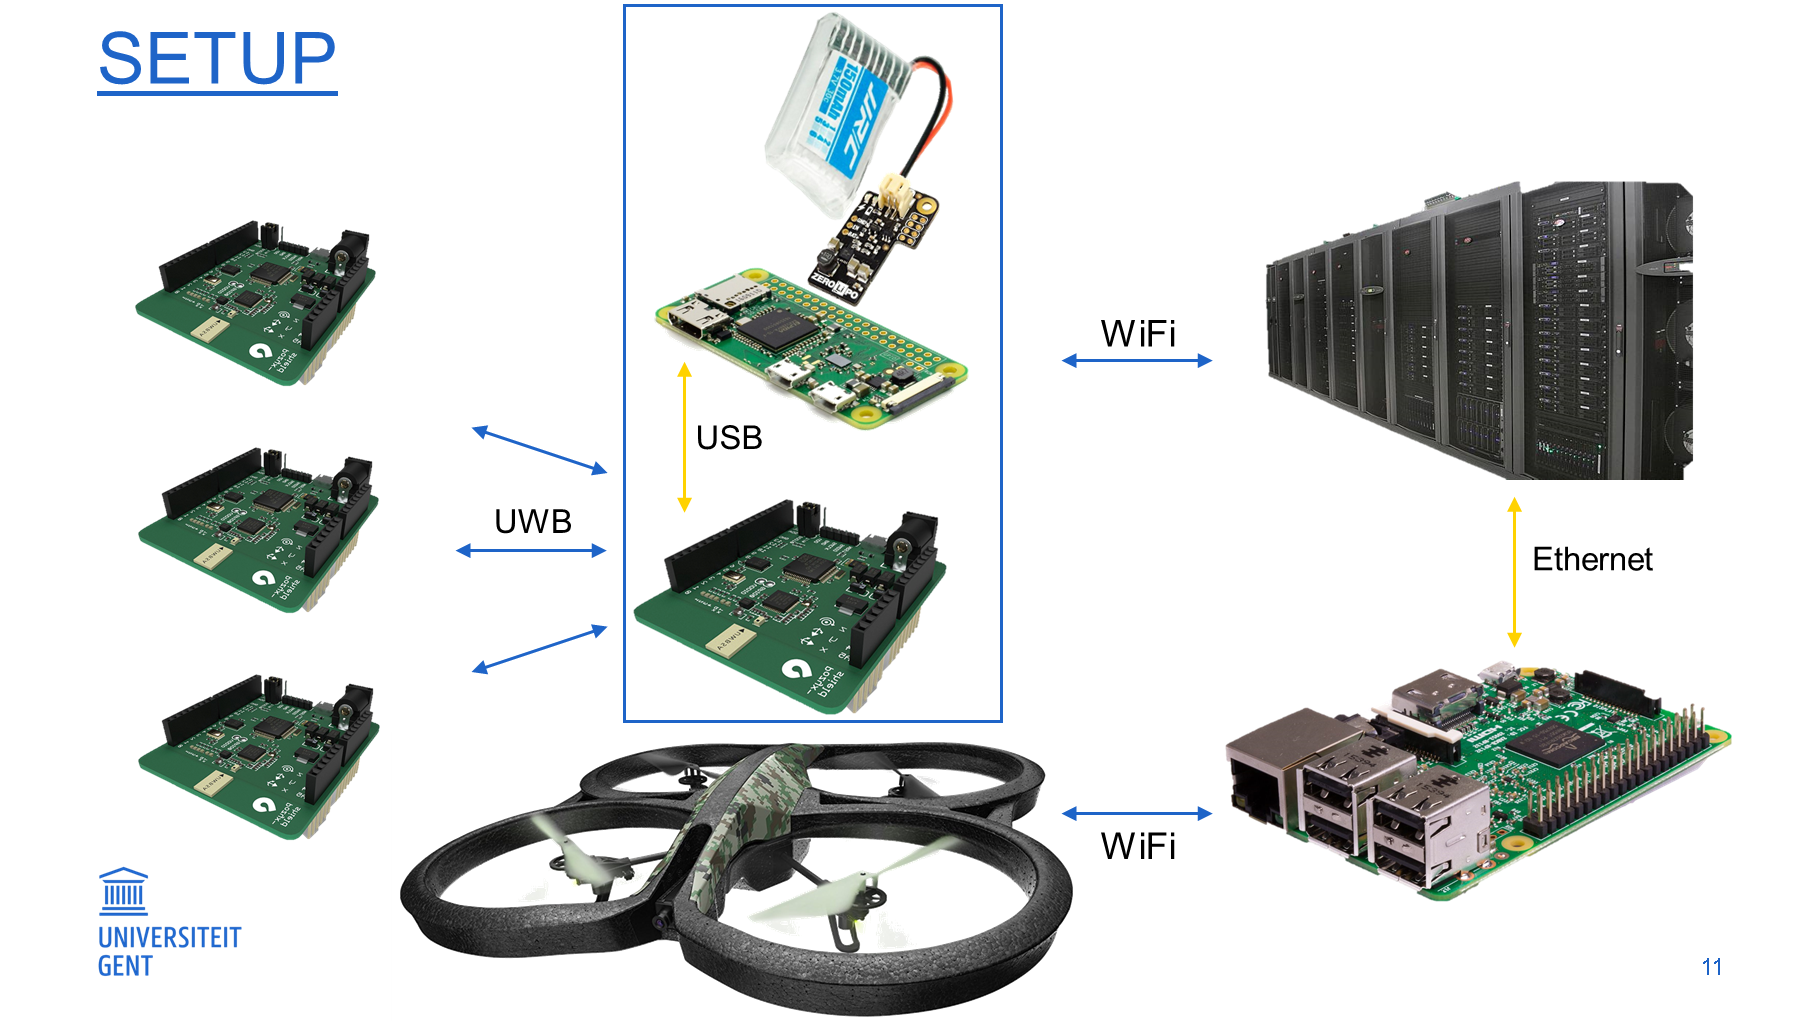
\includegraphics[width=\textwidth]{Setup_Hardware}
	\caption[Hardware setup]{Hardware setup.}
	\label{fig:setup_hardware}
\end{figure}
